%% used templates
%% https://www.overleaf.com/latex/templates/uct-report-template/grctkzjtrqrm#.WB3uy_nhCUm
%% https://www.overleaf.com/latex/examples/title-page-with-logo/hrskypjpkrpd#.WB3uxPnhCUl
%% 

\documentclass[12pt]{article}
\usepackage[english, ngerman]{babel}
\usepackage{natbib}
\usepackage{url}
\usepackage[utf8x]{inputenc}
\usepackage{amsmath}
\usepackage{graphicx}
\usepackage{parskip}
\usepackage{fancyhdr}
\usepackage{vmargin}
\usepackage{lipsum}

\usepackage{hyperref} 
\usepackage[figure]{hypcap} 

% Select what to do with todonotes: 
% \usepackage[disable]{todonotes} % notes not showed
\usepackage[draft]{todonotes}   % notes showed

\setmarginsrb{3 cm}{2.5 cm}{3 cm}{2.5 cm}{1 cm}{1.5 cm}{1 cm}{1.5 cm}

\title{Entwicklung eines Rahmenwerks zur Realisierung von Videospielklassikern} % Title
\author{Joan-Angelo Douvere} % Author
\date{\today} % Date

\makeatletter
\let\thetitle\@title
\let\theauthor\@author
\let\thedate\@date
\makeatother

\pagestyle{fancy}
\fancyhf{}
\rhead{\begin{flushright}\theauthor\end{flushright}}
\lhead{Entwicklung eines Rahmenwerks zur Realisierung von\newline Videospielklassikern - Space Panic}
\cfoot{\thepage}

\begin{document}

%%%%%%%%%%%%%%%%%%%%%%%%%%%%%%%%%%%%%%%%%%%%%%%%%%%%%%%%%%%%%%%%%%%%%%%%%%%%%%%%%%%%%%%%%

\begin{titlepage}
	\centering
    \vspace*{0.5 cm}
    
\includegraphics[scale = 0.25]{images/Hska_logo}\\[1.0 cm]
    \textsc{\LARGE Projektarbeit}\\[2.0 cm]
	\textsc{\Large Informatik}\\[0.5 cm]
	\textsc{\large Bachelor}\\[0.5 cm]
	\rule{\linewidth}{0.2 mm} \\[0.4 cm]
	{ \huge \bfseries \thetitle}\\ [0.3 cm]
    { \LARGE \bfseries \textit{Space Panic}}\\
	\rule{\linewidth}{0.2 mm} \\[1.5 cm]
    
	
	\begin{minipage}{0.4\textwidth}
		\begin{flushleft} \large
			\emph{Autor:}\\
			\theauthor
			\end{flushleft}
			\end{minipage}~
			\begin{minipage}{0.4\textwidth}
			\begin{flushright} \large
			\emph{Betreuer:} \\
			Prof. Dr. Christian Pape
		\end{flushright}
	\end{minipage}\\[2 cm]
	
	{\large \thedate}\\[2 cm]
 
	\vfill
	
\end{titlepage}

%%%%%%%%%%%%%%%%%%%%%%%%%%%%%%%%%%%%%%%%%%%%%%%%%%%%%%%%%%%%%%%%%%%%%%%%%%%%%%%%%%%%%%%%%
%\begin{abstract}
%        \noindent\lipsum[1]
%\end{abstract}
    
\tableofcontents
%\pagebreak

%%%%%%%%%%%%%%%%%%%%%%%%%%%%%%%%%%%%%%%%%%%%%%%%%%%%%%%%%%%%%%%%%%%%%%%%%%%%%%%%%%%%%%%%%

\section{Vorwort}
	Ziel dieser Projektarbeit ist die \textit{Entwicklung eines Rahmenwerks zur Realisierung von Videospielklassikern}. Zur Erreichung dieses Ziels soll ein Klon des Videospiels \textit{Space Panic} aus dem Jahre 1980 realisiert werden. Dieser Bericht beinhaltet die zur Realisierung notwendige Beschreibung des Spiels \textit{Space Panic} und dessen Architektur, sowie meinen Entwurf des Klons und dessen anschließende Implementierung.
    
\section{Anforderungen}
\subsection{Beschreibung}
	\textit{Space Panic} ist ein Arcade-Spiel, das in den 80er Jahren produziert wurde. Die ursprüngliche Version stammt dabei von Universal Co. Ltd. aus dem Jahre 1980 \cite{arcade-museum:space-panic}. Chris Crawford betitelte Space Panic als den Urvater aller Plattformspiele \cite[S. 19]{Crawford:2003:CCG:940762}, da es bereits ein Jahr vor Donkey Kong in den Arcade-Hallen erschien, und somit unverkennbar als Vorbild zahlreicher anderer Spiele desselben Genres diente.
    
	Die Bezeichnung Plattformspiel wird synonym mit Jump'n'Run verwendet. Da jedoch Space Panic die Sprung-Fähigkeit fehlt, bleibt der Titel des ersten Jump'n'Runs Donkey Kong vorbehalten, welches rund acht Monate später veröffentlicht wurde \cite{kotaku:releasedate-dk}.

%%%%%%%%%%%%%%%%%%%%%%%%%%%%%%%%%%%%%%%%%%%%%%%%%%%%%%%%%%%%%%%%%%%%%%%%%%%%%%%%%%%%%


\subsection{Spielprinzip}
	Der Spieler steuert den sogenannten Spaceman, eine menschliche Figur in einem Weltraumanzug.
    
    Technisch bedingt existieren vermutlich maximal 256 verschiedene Level. Allerdings nimmt der Schwierigkeitsgrad so schnell zu, dass ein Fortfahren bereits nach spätestens 30 Levels unmöglich sein sollte.
    
	Jedes Level hat ein indirektes Zeitlimit. Die verbleibende Zeit wird als Sauerstoffvorrat angegeben. Nachdem der eigentliche Sauerstoffvorrat verbraucht ist, kann noch einige Sekunden lang mit einem Notvorrat weitergespielt werden. Während dieser Zeit wird der Kopf des Spacemans rot dargestellt, um den Spieler auf den Sauerstoffmangel hinzuweisen. In späteren Levels erhöht sich die Menge an Sauerstoff, die zu Beginn des Levels verfügbar ist. Mit jeder halben Sekunde nimmt die Menge an Sauerstoff um einen Wert von 20 ab.
    
	Es gibt drei verschiedene Monsterarten, die den Spieler jagen. Jede Monsterart (außer der höchsten) kann unter bestimmten Bedingungen zur nächsthöheren Monsterart evolutionieren. Siehe auch Abschnitt \ref{ssec:Monster}. 
    
    Der Spieler verdient Punkte, indem er Monster tötet. Alle Monsterarten unterscheiden sich in der Art, wie der Spieler sie töten kann, und in der Anzahl der Punkte, die er dafür erhält. Schlüsselelement ist dabei das Graben von Löchern. Siehe auch Abschnitt \ref{ssec:Monster}.
    
    Zusätzlich kann der Spieler Bonuspunkte verdienen, indem er ein Level abschließt, bevor sein Sauerstoffvorrat aufgebraucht ist. Die Restmenge wird dann dem Punktekonto gutgeschrieben.
    
    Der Spieler verliert Leben, wenn er von einem Monster berührt wird oder wenn sein Sauerstoffvorrat vollständig ausläuft.
    
    Ein Spiel gilt als verloren, wenn der Spieler keine Leben mehr hat. Der Spieler kann jedoch einmalig ein Bonus-Leben erhalten, wenn er mehr als 3000 Punkte während des Spiels verdient. 
    
    Ein Level gilt als gewonnen, wenn alle Monster darin getötet wurden. Nachdem ein Level gewonnen wurde, werden dem Spieler die bereits erwähnten Bonuspunkte zugerechnet und das nächste Level beginnt.
    
    Je mehr Levels gewonnen werden, desto schwieriger wird die Zusammenstellung aus Monstern, die sich dem Spieler gegenüberstellen.
    
    Nach einem verlorenen Spiel kann der Spieler seinen Namen eingeben, falls er mit seiner Punktzahl die bisher höchste Punktzahl geschlagen hat. Sein Name erscheint dann mittig auf jedem Bildschirm am oberen Bildschirmrand. Danach landet er wieder auf dem Titelbildschirm.
    
    Das Spiel kann auch durch zwei Spieler gespielt werden, indem jeder Spieler abwechselnd versucht jeweils mehr Punkte als sein Gegenspieler zu erhalten. Gewonnen hat derjenige, der die meisten Punkte am Ende des Spiels verdient hat.
    
\subsection{Bildschirmelemente}
      \begin{figure}[ht!]
          \centering
          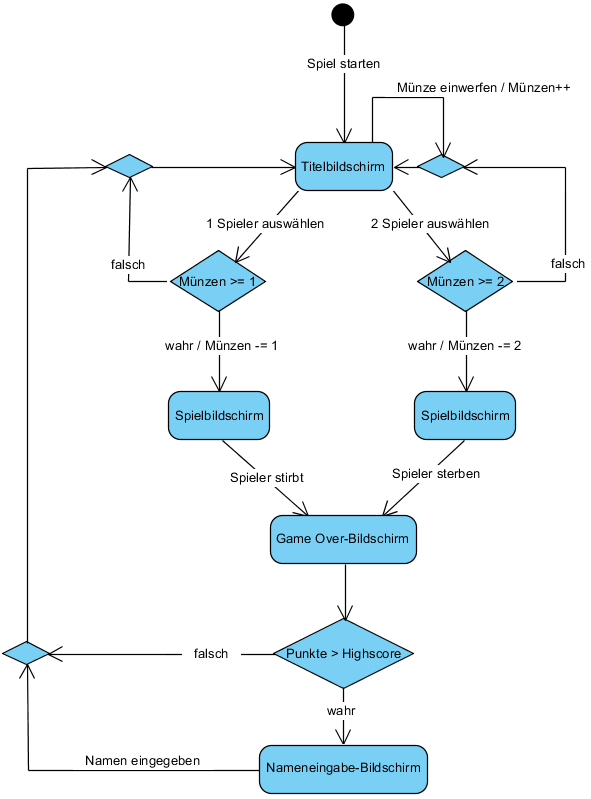
\includegraphics[width=250pt]{images/state_machine}
          \caption{Darstellung der Bildschirme als Zustandsautomat}
          \label{fig:spacepanic:statemachine}
      \end{figure}
Alle Bildschirme (siehe Abb. \ref{fig:spacepanic:statemachine}) teilen sich in drei unterschiedliche Bereiche auf (siehe Abb. \ref{fig:spacepanic:gamescreen}):
\begin{enumerate}
	\item \textbf{Punktebereich} (Oben) \newline
  		Dieser Bereich besteht aus drei Komponenten:
        \begin{itemize}
            \item Letzter Punktestand von Spieler 1
            \item Letzthöchster Punktestand, sowie der dazugehörige Spielername
            \item Letzter Punktestand von Spieler 2
        \end{itemize}
	\item \textbf{Inhaltsbereich} (Mitte) \newline
		Dieser Bereich zeigt dem Spieler den eigentlichen Inhalt des Bildschirms. 
	\item \textbf{Statusbereich} (Unten) \newline
		Dieser Bereich zeigt dem Spieler Statusinformationen zum aktuellen Bildschirm.
\end{enumerate}

\begin{figure}[ht!]
          \centering
          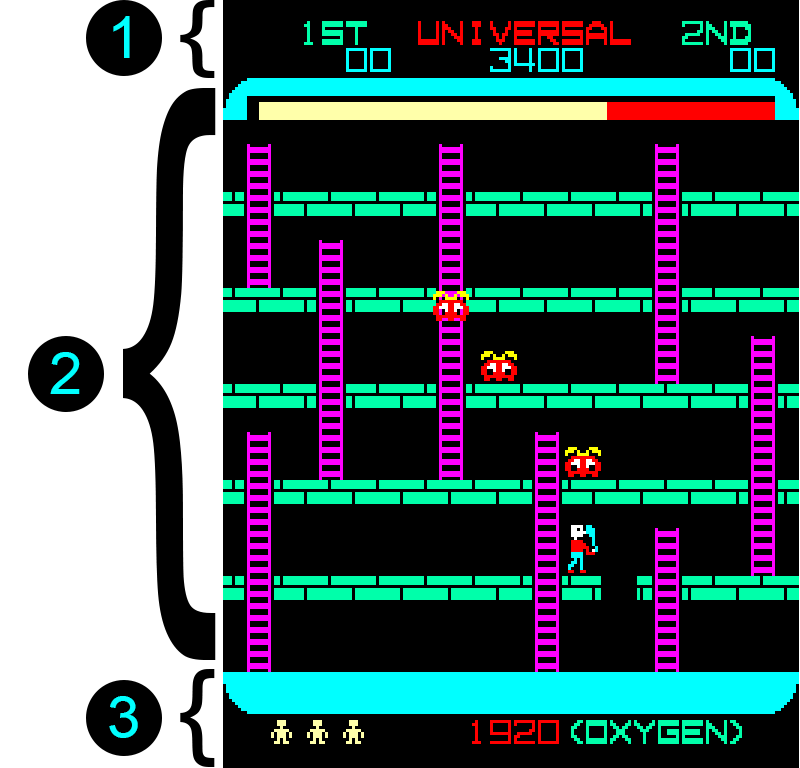
\includegraphics[height=180pt]{images/spielbildschirm_mit_legende}
          \caption{Der Bildschirm von \textit{Space Panic} während einer laufenden Spielrunde. \newline 1. Punktebereich, 2. Inhaltsbereich, 3. Statusbereich}
          \label{fig:spacepanic:gamescreen}
      \end{figure}


%%%%%%%%%%%%%%%%%%%%%%%%%


\subsubsection{Titelbildschirm} \label{ssec:titlescreen}
Auf diesem Bildschirm befindet sich der Spieler, nachdem die Arcade-Maschine gestartet wurde (siehe Abb. \ref{fig:spacepanic:titlescreen}). Wirft man eine Münze ein und startet ein Spiel, erscheint der Spielbildschirm (siehe Abschnitt \ref{ssec:gamescreen}).

	
\begin{enumerate}
    \item \textbf{Inhaltsbereich} (Mitte) \newline
    	Hier sehen potenzielle Spieler einen großzügig angelegten Schriftzug mit dem Titel des Spiels und etwas kleiner einen Spielhinweis zur weiteren Motivation. Weiter unten sehen sie noch den Urheberrechtshinweis des Spielproduzenten.
    \item \textbf{Statusbereich} (Unten) \newline
    	Hier wird die restliche Anzahal an Spielen angezeigt, die noch gespielt werden können. Für jede weitere eingeworfene Münze erhält man ein weiteres Spiel.
\end{enumerate}
\begin{figure}[ht]
		\centering
        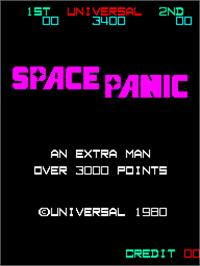
\includegraphics[height=180pt]{images/titlescreen}
        \caption{Der Titelbildschirm von \textit{Space Panic}}
        \label{fig:spacepanic:titlescreen}
	\end{figure}

%%%%%%%%%%%%%%%%%%%%%%%%%%%%%%%%%%%%

\subsubsection{Spielbildschirm} \label{ssec:gamescreen}
	Auf diesem Bildschirm wird das Spiel gespielt. Sind alle Leben aufgebraucht, wechselt das Spiel auf den Spielende-Bildschirm (siehe Abschnitt \ref{ssec:gameoverscreen}).
    
	(Siehe Abb. \ref{fig:spacepanic:gamescreen})
\begin{enumerate}
\item \textbf{Inhaltsbereich} (Mitte) \newline
Hier interagiert der Spieler mit der Spielwelt. Am oberen Rand wird ihm die restliche Zeit, bevor ihm sein Sauerstoffvorrat ausgeht, als Balkengrafik angezeigt. Der Balken besteht aus einem gelben Anteil, der die  und einem roten Anteil. Läuft der gelbe Anteil aus, ist der Sauerstoffvorrat des Weltraumanzugs aufgebraucht und der Spieler kann noch einige Sekunden mit einer Notreserve, dem roten Anteil, spielen. Während die Notreserve benutzt wird, leuchtet der Kopf der Spielfigur rot. 


\item \textbf{Statusbereich} (Unten) \newline
Hier werden dem Spieler seine verbleibenden Leben und sein restlicher Sauerstoffvorrat angezeigt.

Die Anzahl an Leben reicht von 0 bis 4, der Sauerstoffvorrat von 0 bis 4000 (siehe Tabelle \ref{table:oxygen-per-level}).
\end{enumerate}
    
\begin{table}[ht]
\centering
\begin{tabular}{llll}
\hline
\textbf{Level} & \textbf{Sauerstoffmenge (Spielzeit)} & \textbf{Reservezeit} & \textbf{Gesamtspielzeit} \\ \hline
1-3            & 2000 (ca. 90 Sekunden)               & ca. 15 Sekunden      & ca. 105 Sekunden                   \\
4-6            & 3000 (ca. 135 Sekunden)              & ca. 15 Sekunden      & ca. 150 Sekunden                   \\
7-n            & 4000 (ca. 180 Sekunden)              & ca. 15 Sekunden      & ca. 195 Sekunden                   \\ \hline
\end{tabular}
\caption{Sauerstoffmenge und Spielzeit pro Level}
\label{table:oxygen-per-level}
\end{table}
    
%%%%%%%%%%%%%%%%%%%%%%%%%%%%%%%%%%%%%%    
    
\subsubsection{Game Over-Bildschirm} \label{ssec:gameoverscreen}

\begin{figure}[ht]
		\centering
        
\includegraphics{images/game-over}
        \caption{Der GAME OVER-Schriftzug beim Spielende}
        \label{fig:spacepanic:gameover}
	\end{figure}

Wenn das Spiel endet, blendet sich der Schriftzug \mbox{GAME OVER} mittig über dem Spielbildschirm ein (siehe Abb. \ref{fig:spacepanic:gameover}). Das besondere an diesem ist, dass jeder Buchstabe der Farbe des Hintergrunds an der Stelle entspricht. Das heißt, dass ein Buchstabe über einer Leiter violett und ein Buchstabe über einem Stein grün dargestellt wird. Löcher werden dabei als Steine interpretiert.

  \begin{figure}[ht]
		\centering
        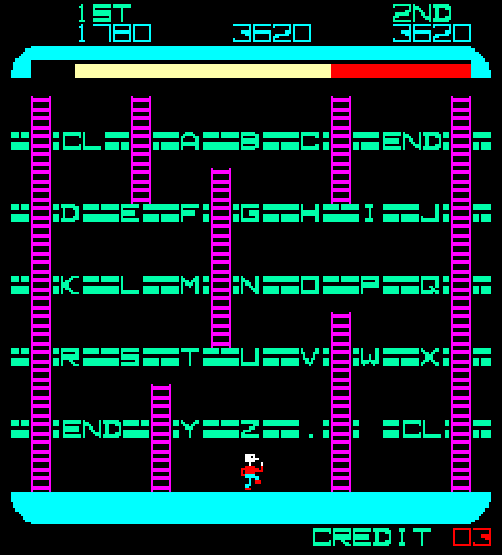
\includegraphics[height=180pt]{images/entername}
        \caption{Der Namenseingabe-Bildschirm}
        \label{fig:spacepanic:entername}
	\end{figure}
  
    Wenn der Spieler einen neuen Höchstpunktestand erreicht hat, wird er anschließend auf den Namenseingabe-Bildschirm gebracht (siehe Abschnitt \ref{ssec:entername}).
    
    Wenn der Spieler keinen neuen Höchstpunktestand erreicht hat, wird er zurück auf den Titelbildschirm gebracht (siehe Abschnitt \ref{ssec:titlescreen}).

Dadurch, dass dieser Bildschirm nur ein Overlay über dem Spielbildschirm darstellt, teilt er sich auch dessen Punkte- und Statusbereich.

%%%%%%%%%%%%%%%%%%%%%%%

\subsubsection{Namenseingabe-Bildschirm} \label{ssec:entername}
Auf diesem Bildschirm kann der Spieler seinen Namen eintragen, unter dem seine Punkte gespeichert werden sollen (siehe Abb. \ref{fig:spacepanic:entername}). Der Name wird dann später im jeweiligen Punktebereich auf sämtlichen Bildschirmen angezeigt.

\begin{enumerate}
\item \textbf{Inhaltsbereich} (Mitte) \newline
Dieser ähnelt stark dem Inhaltsbereich des Spielbildschirms (siehe Abb. \ref{fig:spacepanic:gamescreen} und hat die Besonderheit, dass man sich auf ihm wie in einem laufenden Spiel bewegen kann.

Die Buchstaben und Steuertasten werden als Steine dargestellt und der Spieler muss auf ihnen graben, um sie zu betätigen.

Eine weitere Besonderheit ist, dass auch dieses Level zeitlich begrenzt ist. Nach Ablauf der Zeit, oder nach Betätigung der END Schaltfläche wird der Name gespeichert und der Spieler auf den Titelbildschirm weitergeleitet (siehe Abschnitt \ref{ssec:titlescreen}).

\item \textbf{Statusbereich} (Unten) \newline
	Dieser gleicht dem Statusbereich des Titelbildschirms (siehe Abschnitt \ref{ssec:titlescreen}), indem hier die verbleibenden Spielversuche angegeben werden.
\end{enumerate}




\subsection{Leveldesign}
	Jedes Level besteht aus sechs Ebenen, die durch Leitern verbunden sind. Die Anordnung und Länge der Leitern wird für jedes Level und nach jedem Tod des Spielers zufällig aus einer vordefinierten Menge ausgewählt. 
    
    Eine Leiter verbindet mindestens zwei Ebenen. Ebenen können unterbrochen werden, indem der Spieler darin ein Loch gräbt, und wieder verbunden werden, indem er die Löcher wieder schließt. Wenn der Spieler über ein Loch läuft, fällt dieser hinein. Wenn ein Monster über ein Loch läuft, wird dieses darin gefangen.


%%%%%%%%%%%%%%%%%%%%%%%%%

\subsection{Monster} \label{ssec:Monster}
	Monster jagen die Spielfigur und versuchen sie zu töten, indem sie sie berühren.
    
    Bei einer Berührung mit der Spielfigur verliert dieser ein Leben.
    
    Läuft ein Monster in ein Loch, so bleibt es dort stecken, aber nur, wenn dort noch kein anderes Monster steckt. Gräbt der Spieler das Loch gerade von der anderen Seite zu, so wartet das Monster bis der Spieler fertig ist.
    
    Wird ein Monster in einem Loch zugegraben, so fällt es herunter. Je nach Monsterstufe, stirbt ein Monster wenn es mindestens eine, zwei oder drei Ebenen tief fällt (siehe Tabelle \ref{table:monsterscores}).
    
    Fällt ein Monster auf ein anderes Monster, so sterben beide. Die Punktzahl beider Monster wird dabei addiert. 
    
    Fällt ein Monster nicht nach spätestens drei Sekunden, so klettert es wieder drei Sekunden lang aus dem Loch und evolutioniert zur nächsten Stufe. Während es herausklettert, kann es noch begraben werden.
    
    Die Spielfigur muss alle Monster töten, um eine Spielrunde zu gewinnen.
    
    Je höher die Monsterstufe, desto hartnäckiger verfolgt das Monster den Spieler.
    
\begin{table}[ht]
\centering
\begin{tabular}{c|ccc|}
\cline{2-4}
                                                     & 
\includegraphics{images/monster} & 
\includegraphics{images/boss} & 
\includegraphics{images/don} \\
\textbf{}                                            & \textbf{Monster} & \textbf{Boss} & \textbf{Don} \\ \hline
\multicolumn{1}{|l|}{fällt durch 1 Ebene}  & 100                        & (stirbt nicht)    & (stirbt nicht)   \\ \hline
\multicolumn{1}{|l|}{fällt durch 2 Ebenen} & 200                        & 300                     & (stirbt nicht)   \\ \hline
\multicolumn{1}{|l|}{fällt durch 3 Ebenen} & 400                        & 600                     & 800                    \\ \hline
\multicolumn{1}{|l|}{fällt durch 4 Ebenen} & 800                        & 1200                    & 1600                   \\ \hline
\multicolumn{1}{|l|}{fällt durch 5 Ebenen} & 800                        & 1200                    & 2000                   \\ \hline
\end{tabular}
\caption{Punkte beim Töten von Monstern}
\label{table:monsterscores}
\end{table}    

%%%%%%%%%%%%%%%%%%%%%


\subsection{Animation}
Die Animationen von Space Panic sind sehr schlicht gehalten. Jede Animation besteht aus 2 Einzelbildern.

Folgende Animationen existieren:
\begin{enumerate}
\item Spieler läuft zur Seite (andere Richtung gespiegelt)
\item Spieler klettert
\item Spieler gräbt
\item Monster läuft / fällt / klettert
\item Monster steckt in Loch
\end{enumerate}

%%%%%%%%%%%%%%%%%%%%%%%%%
    
\subsection{Sounddesign}
Das Sounddesign von Space Panic besteht vollständig aus synthetischen Soundeffekten, kodiert als 1-Bit-DAC-Sequenzen. Das fast vollständige Soundpaket findet man u.a. auf MAMEWorld \cite[panic.zip]{mameworld:samples}. Die restlichen Sounds und Musiksequenzen finden sich u.a. in diversen Videos auf YouTube \cite{youtube:spacepanic1}.

Folgende Soundeffekte existieren im Spiel:
\begin{itemize}
\item Spieler oder Monster erscheint auf dem Bildschirm
\item Spieler läuft
\item Spieler klettert
\item Spieler gräbt
\item Spieler stirbt
\item Sauerstoff-Notvorrat wird verwendet
\item Monster befindet sich in einem Loch
\item Spieler oder Monster fällt
\item Monster stirbt
\item Monster klettert aus Loch heraus
\item Monster landet nach einem Fall und stirbt nicht
\end{itemize}

Folgende Musiksequenzen existieren im Spiel:
\begin{itemize}
\item Spieler gewinnt ein Level
\end{itemize}

%%%%%%%%%%%%%%%%%%%%%%%%%%

\section{Entwurf}
	\todo[inline]{Entwurf beschreiben}
    %\lipsum[1-3]
\section{Implementierung}
\todo[inline]{Implementierung beschreiben}
	%\lipsum[2-4]
\section{Reflektion}
\todo[inline]{Unterschiede zum Original beschreiben}
	%\lipsum[5]
%%%%%%%%%%%%%%%%%%%%%%%%%%%%%%%%%%%%%%%%%%%%%%%%%%%%%%%%%%%%%%%%%%%%%%%%%%%%%%%%%%%%%%%%%%%%%
\newpage
\addcontentsline{toc}{section}{Literatur}
\bibliographystyle{plain}
\bibliography{biblist}

\end{document}